\documentclass[14pt]{article}
%General Packages
\usepackage{multicol, enumerate, enumitem, hyperref, color, soul, setspace, parskip, fancyhdr}

%Math Packages
\usepackage{amssymb, amsthm, amsmath, bbm, latexsym, units, mathtools}

%All math in Display Style
\everymath{\displaystyle}

% Packages with additional options
%\usepackage[T1]{fontenc}
\usepackage[headsep=0.5cm,headheight=0cm, left=1 in,right= 1 in,top= 1 in,bottom= 1 in]{geometry}
\usepackage[usenames,dvipsnames]{xcolor}

% SageTeX
\usepackage{sagetex}

% Package to use the command below to create lines between items
\usepackage{dashrule}
\newcommand{\litem}[1]{\item#1\hspace*{-1cm}\rule{\textwidth}{0.4pt}}

\pagestyle{fancy}
\lhead{Module\,2\,-\,Linear\,Functions}
\chead{}
\rhead{Progress Exam 3}
\lfoot{Summer\,C\,2020}
\cfoot{}
\rfoot{Version C}

\begin{document}
\pagestyle{fancy}

\begin{sagesilent}
load("../Code/generalPurposeMethods.sage")
load("../Code/keyGeneration.sage")
keyFileName = "Module2"
version = "C"
\end{sagesilent}

\begin{enumerate}
\setcounter{enumi}{5}


\begin{sagesilent}
moduleNumber=2
problemNumber=6
load("../Code/linear/linearGraphToStandard.sage")
\end{sagesilent}

\litem{ \sage{displayStem}

	\begin{center}
	 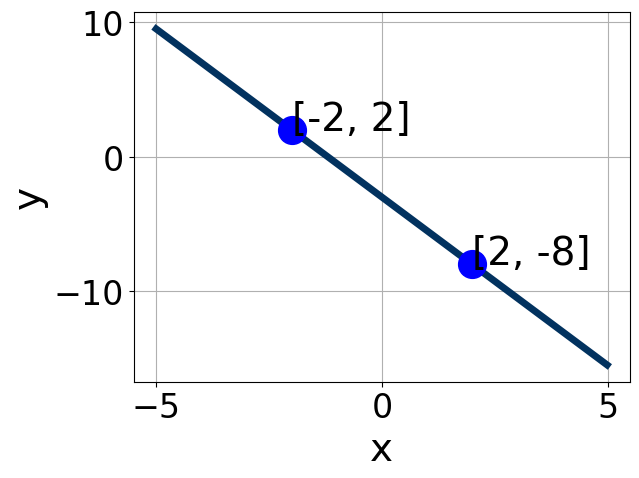
\includegraphics[width=.3\textwidth]{../Figures/linearGraphToStandardC.png}
	 \end{center}

	\begin{enumerate}[label=\Alph*.]
    \item \( \sage{choices[0]} \)
    \item \( \sage{choices[1]} \)
    \item \( \sage{choices[2]} \)
    \item \( \sage{choices[3]} \)
    \item \( \sage{choices[4]} \)
	\end{enumerate}

}

\begin{sagesilent}
moduleNumber=2
problemNumber=7
load("../Code/linear/linearParOrPer.sage")
\end{sagesilent}

\litem{	\sage{displayStem}

\[ \sage{displayProblem} \]

	\begin{enumerate}[label=\Alph*.]
    \item \( \sage{choices[0]} \)
    \item \( \sage{choices[1]} \)
    \item \( \sage{choices[2]} \)
    \item \( \sage{choices[3]} \)
    \item \( \sage{choices[4]} \)
	\end{enumerate}

}

\begin{sagesilent}
moduleNumber=2
problemNumber=8
load("../Code/linear/linearTwoPoints.sage")
\end{sagesilent}

\litem{ \sage{displayStem}

\[ \sage{displayProblem} \]

	\begin{enumerate}[label=\Alph*.]
    \item \( \sage{choices[0]} \)
    \item \( \sage{choices[1]} \)
    \item \( \sage{choices[2]} \)
    \item \( \sage{choices[3]} \)
    \item \( \sage{choices[4]} \)
	\end{enumerate}
}

\begin{sagesilent}
moduleNumber=2
problemNumber=9
load("../Code/linear/solveIntegerLinear.sage")
\end{sagesilent}

\litem{ \sage{displayStem}

  % \( \sage{displayProblem} \)
	\[ \sage{blocks[0]}(\sage{blocks[1]+blocks[2]*x}) = \sage{blocks[3]}(\sage{blocks[4]*x-blocks[5]}) \]

	\begin{enumerate}[label=\Alph*.]
    \item \( \sage{choices[0]} \)
    \item \( \sage{choices[1]} \)
    \item \( \sage{choices[2]} \)
    \item \( \sage{choices[3]} \)
    \item \( \sage{choices[4]} \)
	\end{enumerate}

}

\begin{sagesilent}
moduleNumber=2
problemNumber=10
load("../Code/linear/solveRationalLinear.sage")
\end{sagesilent}

\litem{ \sage{displayStem}

 \[ \sage{displayProblem} \]

	\begin{enumerate}[label=\Alph*.]
    \item \( \sage{choices[0]} \)
    \item \( \sage{choices[1]} \)
    \item \( \sage{choices[2]} \)
    \item \( \sage{choices[3]} \)
    \item \( \sage{choices[4]} \)
	\end{enumerate}

}

\end{enumerate}

\end{document}

